% !TEX root = ../notes_template.tex
\chapter{Blood Flow support of Micro-circulation}\label{chp:blood_flow}
Updated on \today
\minitoc
This chapter covers the blood flow support of micro-circulation, which supports the ECF, which supports skeletal muscle function. Blood flow includes the heart as a muscular pump (cardiac function) and the two vascular circuits that the pump circulates blood through (systemic and pulmonary circulation). All together these components can be referred to as the cardiovascular system (anatomical perspective) or circulation (physiological perspective). 

The supportive role of circulation is reliant on cardiac muscle. The relationship between circulation and cardiac muscle is similar to the relationship between movement and skeletal muscle. Concepts from skeletal muscle such as tension, excitation, regulation and energetics are applicable to cardiac muscle. It is useful to compare and contrast cardiac muscle with skeletal muscle across these concepts while focusing on how the differences enable the act of circulation. However, this is not an attempt to shift the focus from a skeletal muscle approach to a cardiac muscle approach. The primary goal of this chapter is an understanding of circulation in its supportive role for skeletal muscle. Therefore, there is less emphasis on the details cardiac muscle and more emphasis on the act of circulation.\footnotemark\footnotetext{Unlike in Part I where there was more emphasis on the details of skeletal muscle and less emphasis on the various manifestations of the act of movement.} 

% Add something about the importance of the circulation (all the reasons, central importance (vital) for living due to its role in supporting ECF; its importance for muscle function and therefore movement and therefore function based on the immediate needs of aerobic energy transformation. The importance of circulation makes it a highly studied area of physiology. Since it has been highly studied it has several useful models for understanding circulation. After reviewing the important structures for blood flow the chapter introduces several of the useful models (in the form of equations that demonstrate relationships).


\vspace{5mm}

\textbf{Objectives include:}
\begin{enumerate}
    \item Describe how the anatomy of the heart and blood vessels supports circulation. 
    \item Apply Poiseuille Law (equation) to describe the function and possible dysfunction of circulation.
    \item Demonstrate the ability to apply the basic concepts of physiology to the analysis of patient/client problems related to the muscular and  circulatory systems.
    \item Relate the the International Classification of Function (ICF) to describe how physiological systems emerge as function and consider the whole system impact of dysfunction (impairments) (7D21)
    \item Show how to perform cardiovascular tests and measures including: Heart rate and Blood pressure in an isolated practice condition.
    \item
    \item
    \item
    \item
    \item
\end{enumerate}

\section{Structures of Blood Flow}

The heart and the roots of the great vessels occupy the pericardium, which is located in the mediastinum. The sternum, the costal cartilages, and the medial ends of the third to fifth ribs on the left side of the thorax create the anterior border of the mediastinum. It is bordered inferiorly by the diaphragm, posteriorly by the vertebral column and ribs, and laterally by the pleural cavity (which contains the lungs). Specific cardiac structures and vessels and their respective functions are depicted in Figure \ref{fig:Cardiac_Anatomy}.

\begin{figure}[!h]
    \centering
    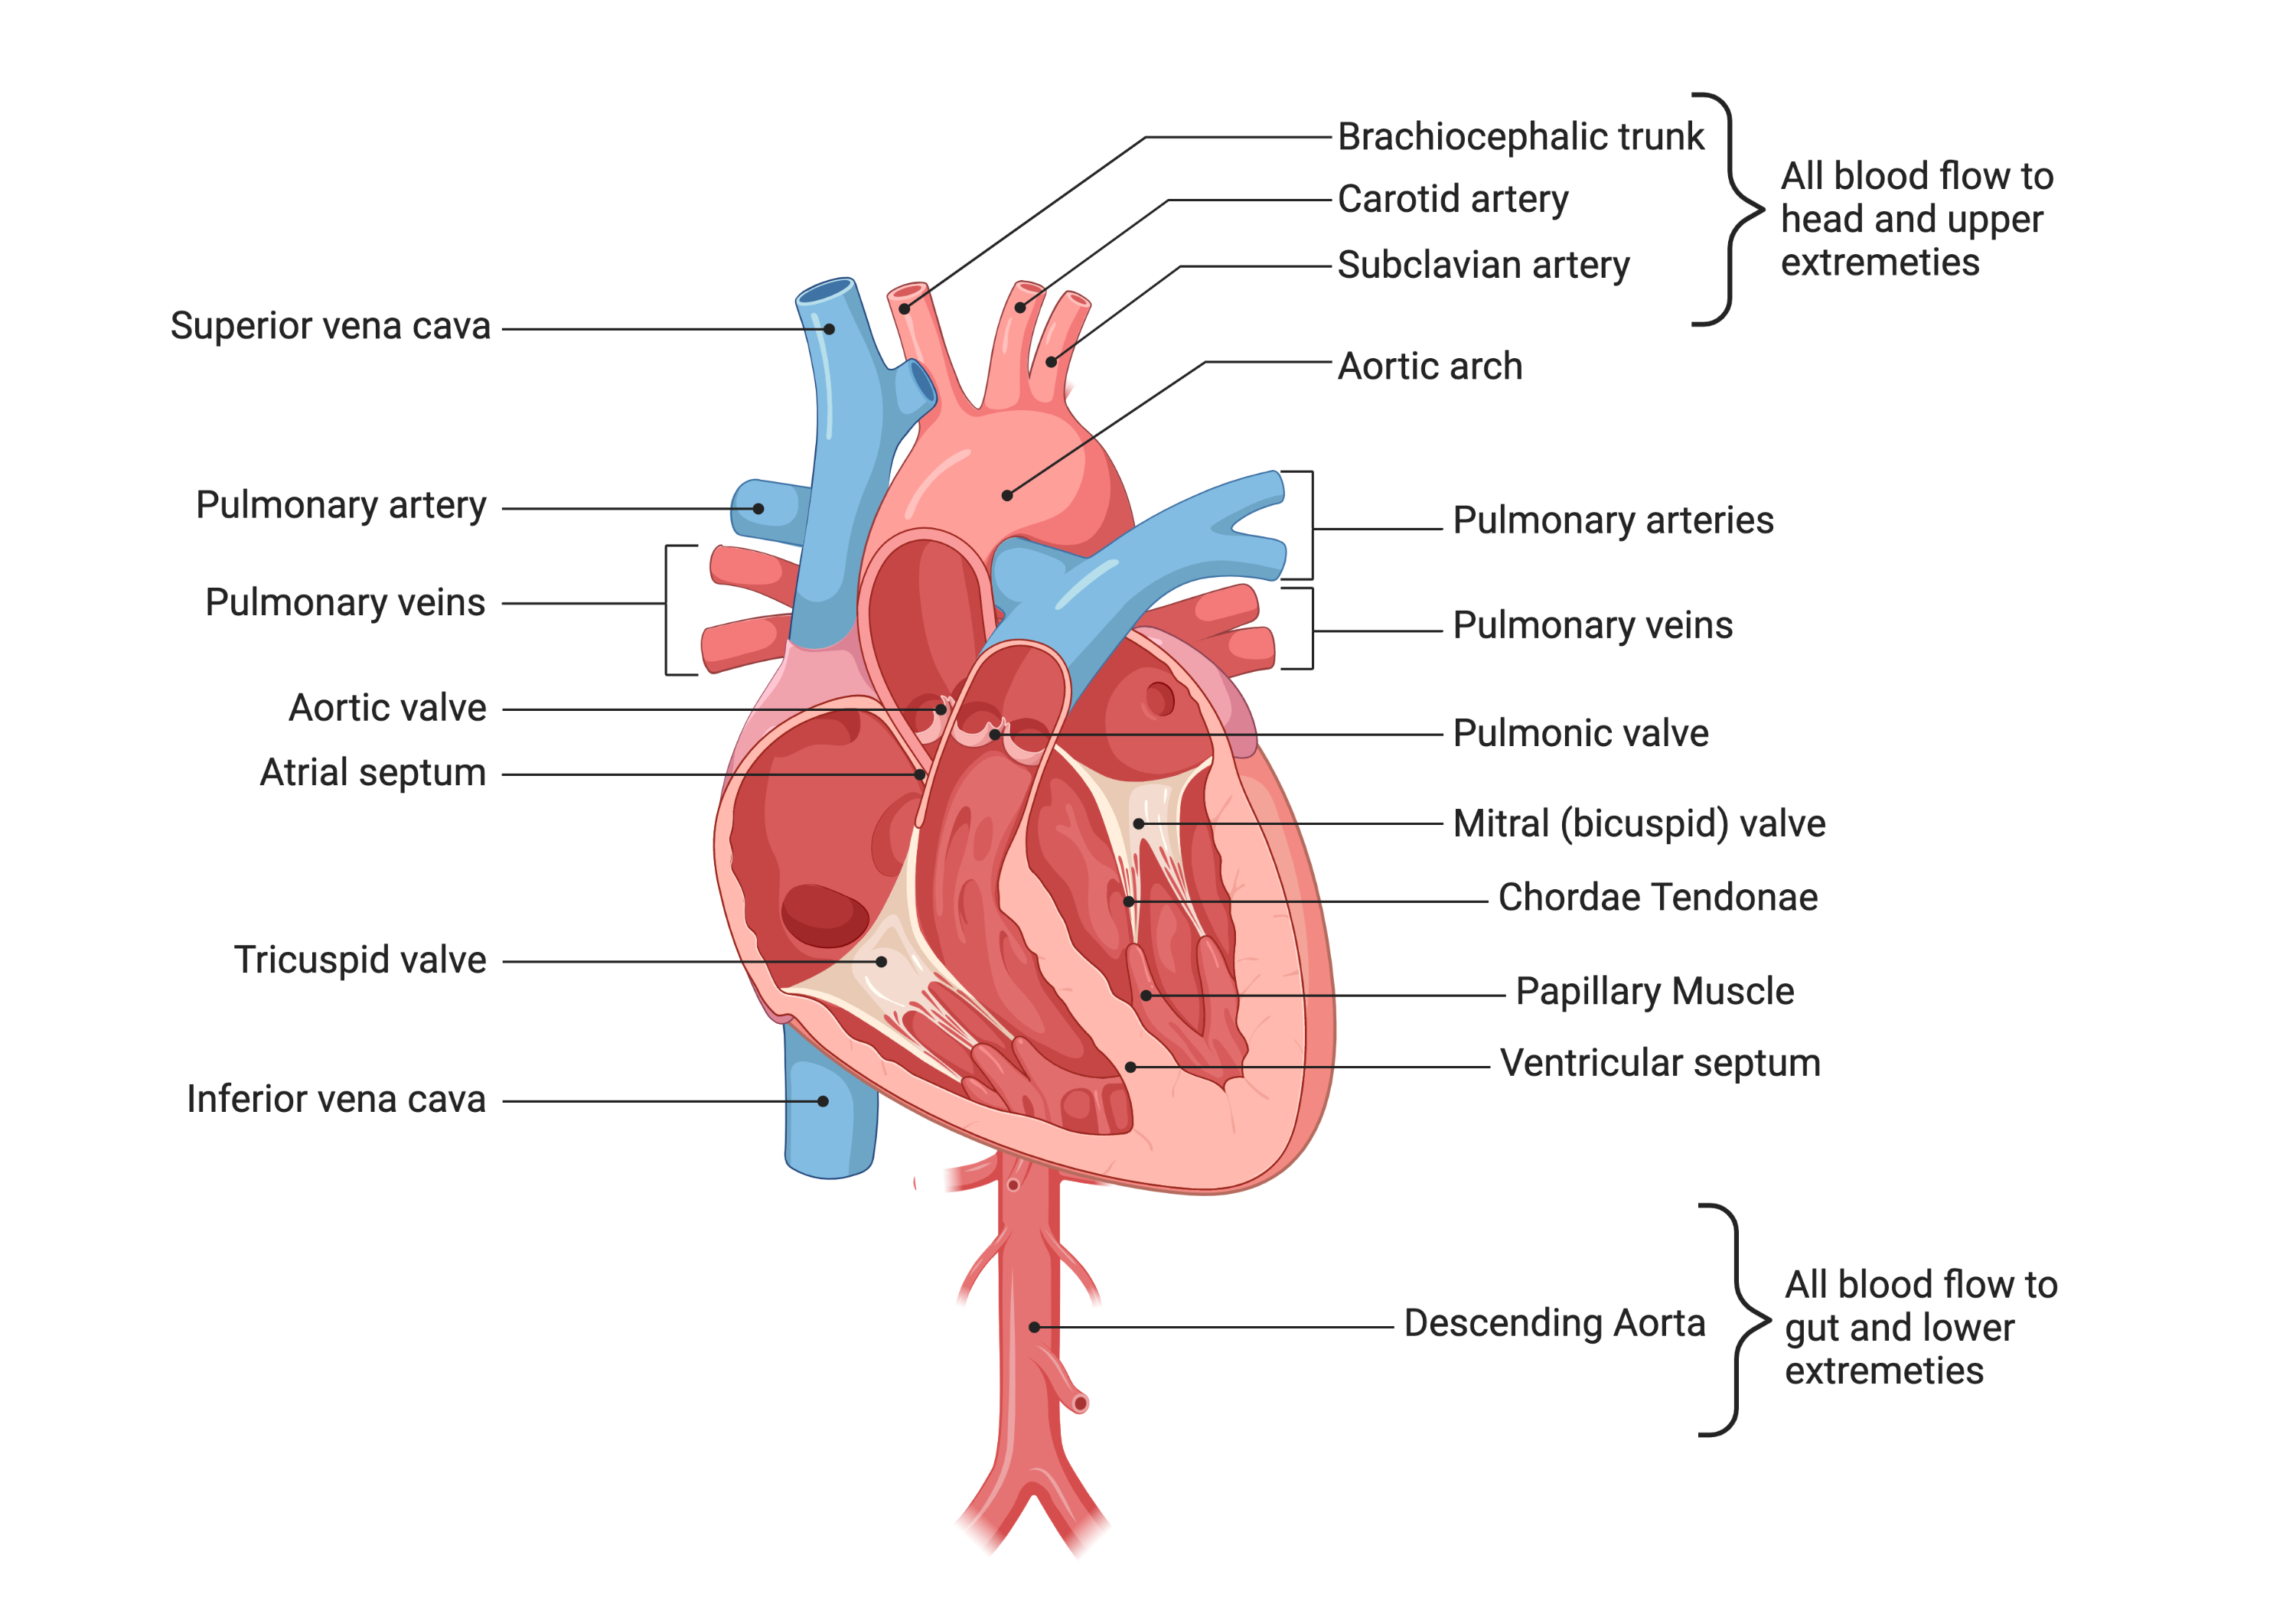
\includegraphics[width=1\linewidth]{./figure/Cardiac_Anatomy.png}
    \caption{Cardiac Anatomy \footnotesize{(Created with BioRender.com)}}
    \label{fig:Cardiac_Anatomy}
\end{figure}

Beyond being familiar with the structure and the names of structures in Figure \ref{fig:Cardiac_Anatomy} that are utilized throughout the chapter, there are several important structural takeaways.

\begin{itemize}
    \item Structurally there are four chambers, right and left atria (RA and LA); right and left ventricle (RV and LV) (the anatomical view).
    \item The four chambers form two primer-pumps for two circulations (right and left), RA and RV for the pulmonary circulation; and LA and LV for the systemic circulation (which includes all skeletal muscles and the heart itself) (the pump view).
    \item The four chambers are divided into two excitation regions, RA and LA for atrial excitation; and RV and LV for ventricular excitation (the excitation view).
    \item Blood flow between the right and left primer-pumps is prevented by a septum (septal wall).
    \item Blood flow direction is guided by four one-way valves (blood flow occurs due to pressure gradients - there is nothing inherently directional about pressure gradients other than high pressure to low pressure - therefore the valves are necessary to keep blood flowing from a chamber to the next chamber and now "backwards").
    \item All blood flow from the gut and lower extremity passes through the descending aorta; and comes to the heart through the inferior vena cava.
    \item All blood flow from the upper extremities and head passes through the great vessels (first three branches off of the aorta); and comes to the heart from the superior vena cava
    \item For blood to flow through the circulation, venous pressure must be lower than arterial pressure
    \item Venous pressure (central in the RA; pulmonary in the LA) refers to the pressure that is the final end point for all venous blood flow returning to the heart which must, for blood flow to occur, have the lowest venous blood pressure of the respective circulations. 
    \item Ventricular systolic pressure refers to the pressure in the ventricles during active tensioning (contraction), for blood flow to occur it must have the highest arterial pressure of the respective circulations. The right sided ventricular systolic pressure is lower than the left sided ventricular systolic pressure, the respective circulations are considered low and high pressure.
    \item Because the ventricular systolic pressures must be the highest through the entire circulation, the tricuspid valve (between the RA and RV) and the bicuspid (mitral) valuve (between the LA and LV) have additional support supplied by the papillary muscles and chordae tendonae (the support does not help them open, it prevents them from allowing backflow while closed).
    \item Because the left ventricle has greater pressure than the right ventricle, the mitral valve papillary muscle and chordae tendonae are more developed
    \item The aortic valve, which is not supported by papillary muscle, is under more pressure than the tricuspid valve because the aortic pressure is the second highest pressure in the circulation, however aortic peak pressure is short lived because of how rapidly blood flows out of the aorta.
\end{itemize}

\section{Blood Flow Overview}

Blood flow is measured and assessed based on the cardiac output ($\dot{Q}$) in liters (or mL) per minute. $\dot{Q}$ is directly proportional to the overall pressure gradient and inversely proportional to resistance to circulation:

\begin{equation}
    \dot{Q} = \frac{P_{arterial} - P_{RA}}{TPR}
    \label{Q}
\end{equation}

Where $P_{arterial}$ is pressure in the arteries (highest in the aorta); $P_{RA}$ is central venous pressure in the RA (lowest in the systemic circulation and normally approximates 0); and $TPR$ is the total peripheral resistance.

Since $P_{RA}$ normally approximates 0, the equation can be simplified to:

\begin{equation}
    \dot{Q} = \frac{P_{a}}{TPR}
    \label{Q_simplified}
\end{equation}

This equation can be manipulated to provide the often utilized equation for arterial pressure (blood pressure (BP)):

\begin{equation}
    P_{a} = \dot{Q} \times TPR
    \label{BP}
\end{equation}

To show that blood pressure is directly proportional to cardiac output and total peripheral resistance. 

As a pump the heart has two phases, a filling phase known as diastole, and a pumping phase known as systole. Therefore, $P_{a}$ has two components referred to as diastolic blood pressure (DBP) and systolic blood pressure (SBP). It is useful to consider SBP and DBP separately as well the mean arterial pressure:

\begin{equation}
    MAP = DBP + \frac{1}{3} \times (SBP - DBP)
    \label{MAP1}
\end{equation}

Since pulse pressure ($PP$) = $SBP - DBP$, then Equation \ref{MAP}, can be simplified to:

\begin{equation}
    MAP = DBP + \frac{1}{3} \times PP
    \label{MAP_simplified}
\end{equation}

Something to note in the relationship between SBP, DBP and MAP is that the MAP is a weighted mean and it is weighted by DBP more than SBP. This is because the overall time period that the heart pump, and therefore the entire circulation, is in systole is much shorter than the overall time they are in diastole. With an increase in heart rate (HR) the time in systole becomes proportionally more time but the systolic time interval is relatively unchanged. The change in overall time in systole is based on there being less time in diastole. Despite this there is no modification to the equation for MAP during periods of higher HR.

Poiseuille's Law offers deeper insight into Equation \ref{Q}.

\begin{equation}
    \dot{Q} = \frac{\Delta P \pi r^4}{\eta L}
    \label{Poiseuille}
\end{equation}

In Equation \ref{Poiseuille} $\dot{Q}$ is directly proportional to the pressure gradient as in Equation \ref{Q} as well as to the vessel cross sectional area squared. Area of a vessel is approximated by the area of a circle ($\pi r^2$), where $\pi$ is a constant and $r^2$ is the radius. Since flow is proportional to cross section area squared $(\pi r^2)^2$, it is proportional to radius to the 4th power ($\pi r^4$). $\dot{Q}$ is inversely proportional to the viscosity of the fluid ($\eta$) and the length of the vessel ($L$). 

It should be noticed that Poiseuille's Law includes all the components of Equation \ref{Q}. $\Delta P$ is the pressure gradient between arteries (primarily aorta) and the right atria. Everything else in Equation \ref{Poiseuille} further elucidates components of TPR as resistance.

\begin{equation}
    R = \frac{\eta L}{\pi r^4}
    \label{resistance}
\end{equation}

The most physiologically relevant variables of Equation \ref{Poiseuille} for blood flow are $\Delta P$, $r^4$ and $\eta$. $\pi$ is a constant and can therefore does not contribute to our understanding of how blood flow changes. And for all intents and purposes $L$ is a constant. Though $L$ is one reason why the heart as a pump must increase it's ability to generate tension as we grow, it is pumping blood through greater length and therefore there is more resistance. 

% Left off here - discuss the variables and how they change to change blood flow.....?

Blood flows from high pressure to low pressure. If there is blood flow, there is a pressure gradient. 


Circulation adjusts the amount of blood pumped out of the heart (cardiac output [$\dot{Q \ Liters/minute}$]) to meet the range of energetic transformation needs.


Add cardiac output here with an overview of the factors that influence cardiac output that can be expanded on in later sections

Systole

Diastole




\section{Cardiac Muscle}

The function of the heart as a muscular pump depends on several characteristics of cardiac muscle:

\begin{itemize}
    
    \item Automaticity: The ability to initiate its own excitation
    \item Rhythmicity: The ability to repeat the excitation-activation cycle in synchrony with regularity
    \item Excitability: The ability to respond to excitation with activation
    \item Conductivity: The ability to transmit excitations from cell to cell within the heart
    \item Contractility: The ability to generate a full contractile (shortening) cycle with each excitation
 
\end{itemize}

\begin{figure}[!h]
    \centering
    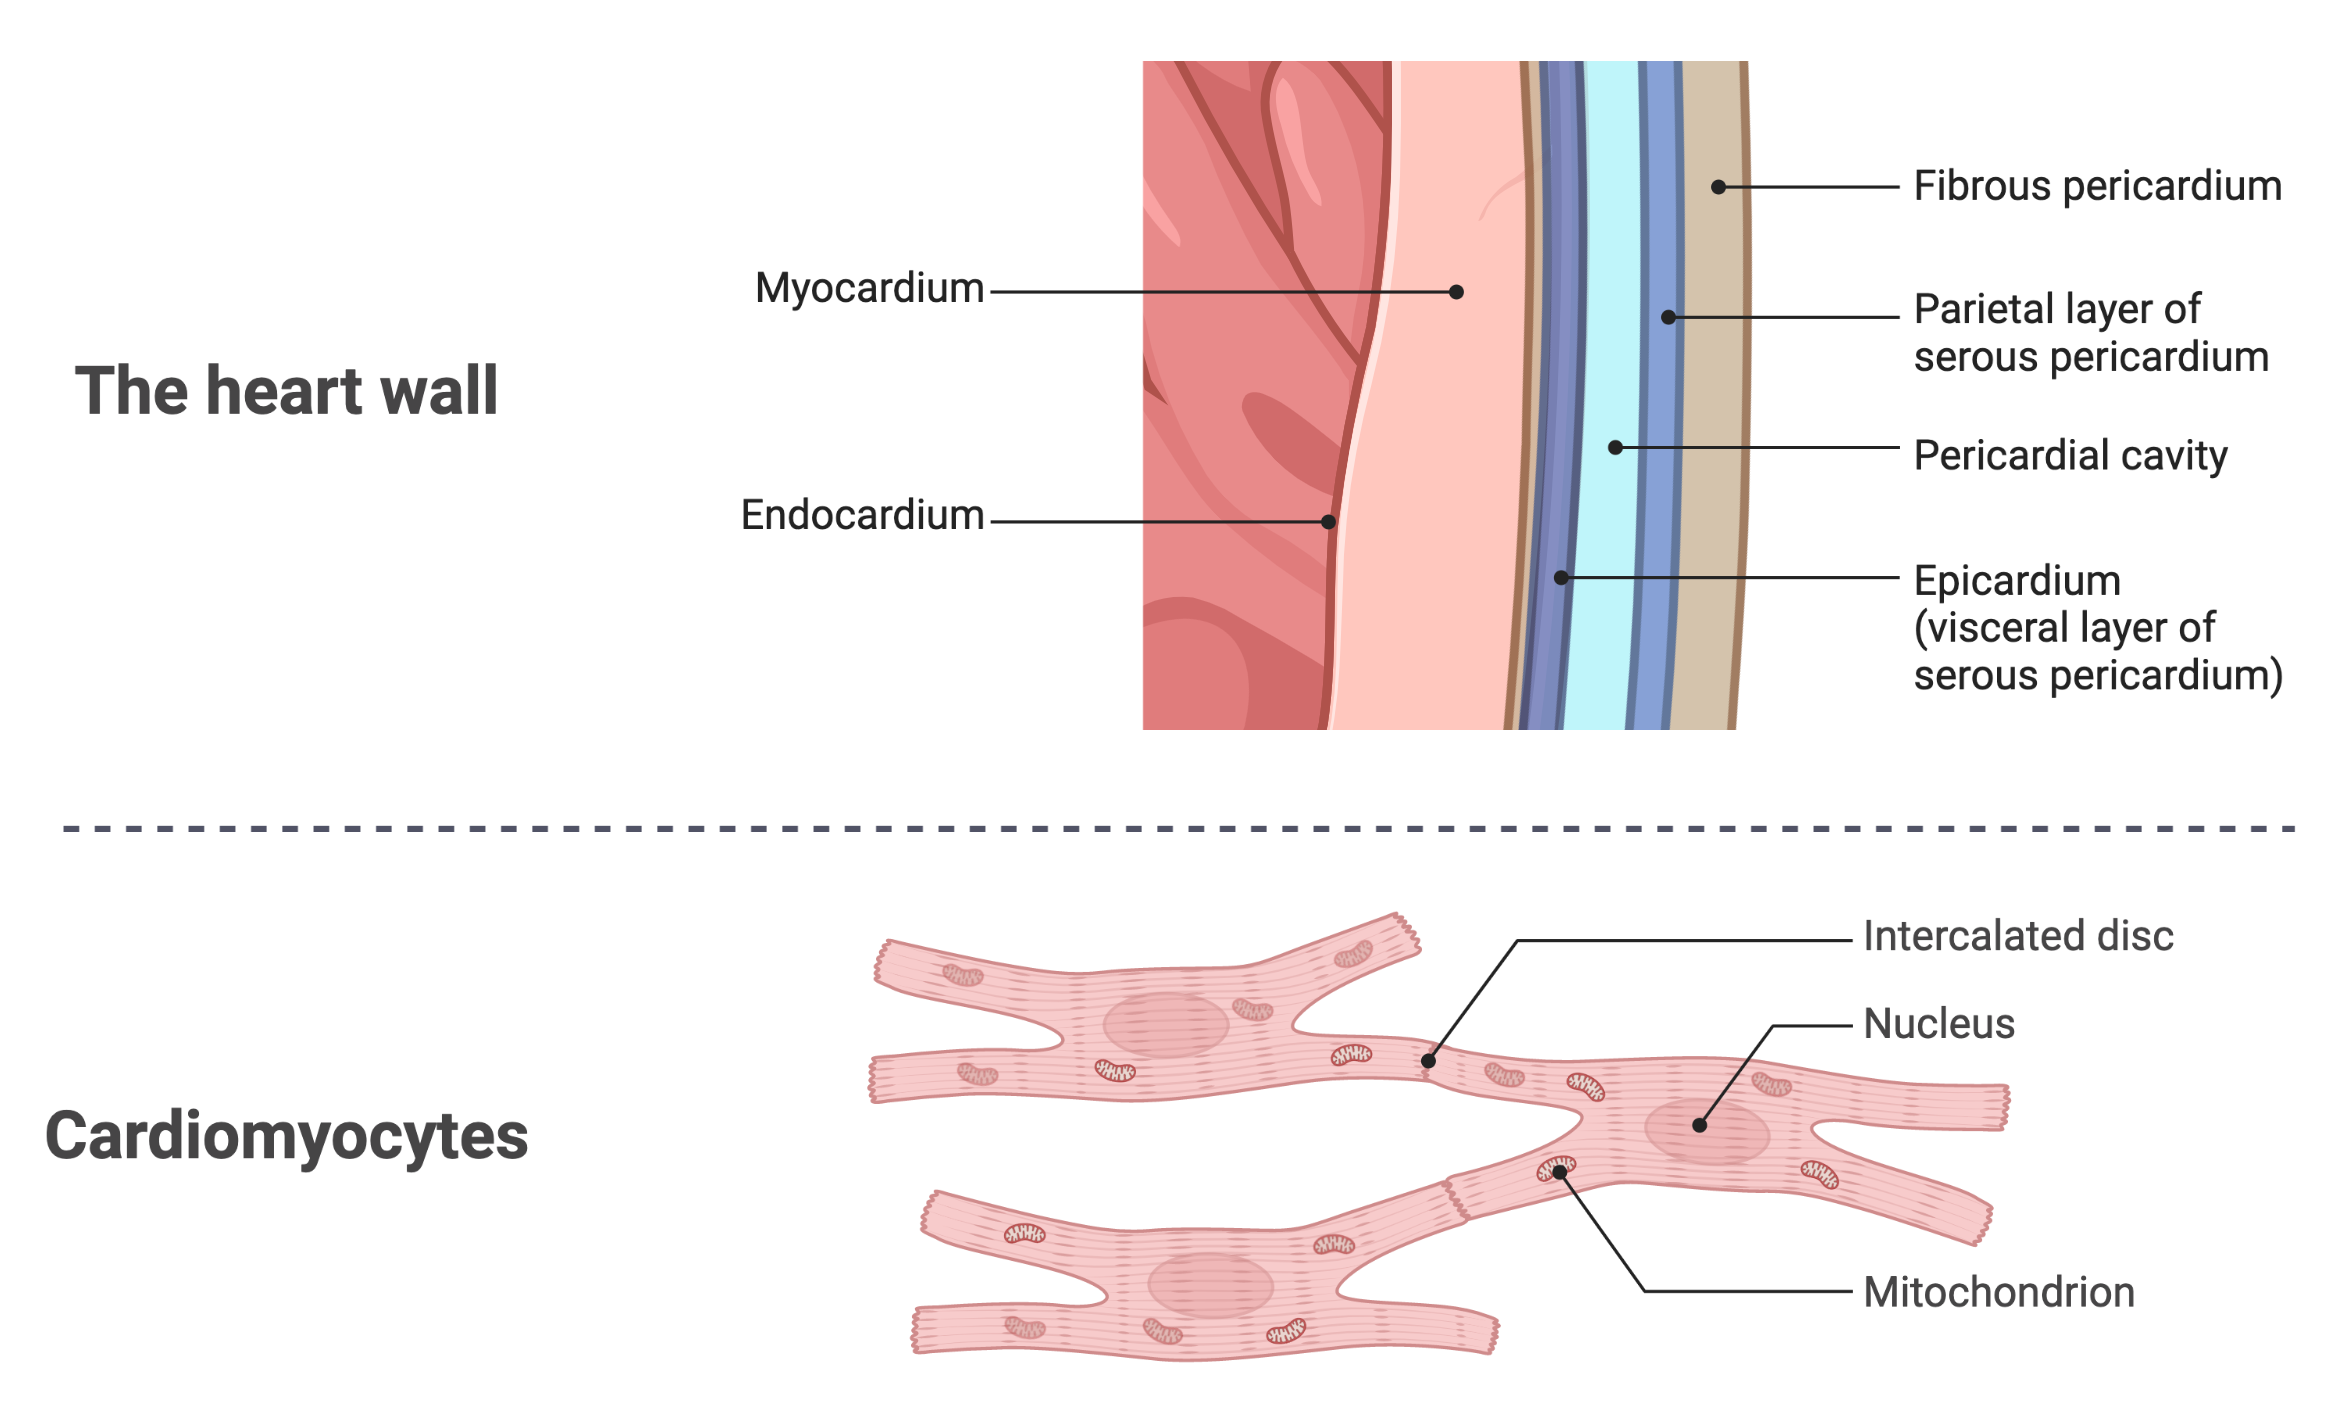
\includegraphics[width=1\linewidth]{./figure/Cardiac_Muscle.png}
    \caption{Cardiac Muscle \footnotesize{(Created with BioRender.com)}}
    \label{fig:Cardiac_Muscle}
\end{figure}

\subsection{Tension}

It is reasonable to use the term contraction when describing activation and active tension for the cardiac muscle because contraction (shortening) is what occurs (there is no eccentric or isometric activation of cardiac muscle). A major difference between cardiac and skeletal muscle is that cardiac muscle does not have a tendon attachment. Cardiac muscle attaches to itself to create a chamber that has a volume. When cardiac muscle contracts, it makes the chamber smaller (less volume). In skeletal muscle the length of fibers directly translates into the length of the entire muscle and this relationship has a functional interpretation. In cardiac muscle the length of fibers directly translates into the volume chambers. It is the volume of these chambers that has functional interpretation. 

The heart has four chambers that function as four pumps (right and left atria; right and left ventricles). However from a muscular perspective there are two chambers, each separated into a right and a left side with a relatively thin muscular barrier between them. This is quite noticeable in conditions that result in abnormal timing of the right and left ventricle excitation. If the ventricles are not excited at the same time, even by a milliseconds, the overall pump effectiveness of both ventricles is impaired.

Active tension is generated in cardiac muscle with the same sliding filament model of skeletal muscle described in Chapter \ref{chp:tension}. Active tension generates tension that shortens cardiac muscle fibers and makes the cardiac chambers smaller. Passive tension is generated by titin (primarily) and other connective tissue structures. Passive tension also attempts to shorten cardiac muscle fibers when they are stretched (lengthened fibers when the chamber has a larger volume). 

Cardiac muscle \textit{in situ} has a volume-tension curve that is synonomous with the length-tension curve of skeletal muscle. The volume-tension curve is similar looking to the length-tension curve. The primary difference between the volume-tension and length-tension curves is that the volume-tension passive component is shifted to the left and is steeper. Passive tension starts to develop prior to achieving resting volume and it develops more rapidly. The functional implication is that even under normal resting conditions passive tension contributes to cardiac contraction. And with larger volumes of blood in the chambers the contribution of passive tension rises exponentially.

The passive component of the volume-tension curve is related to cardiac compliance. As described in Chapter \ref{chp:ecf_microcirculation} there is a relationship between volume, compliance and pressure. The cardiac muscles vary the volume of chambers while having a particular compliance (that varies with the passive and active tension) for the purpose of generating pressure. This is a fundamental difference between cardiac and skeletal muscle tension. Skeletal muscle tension changes length based directly on tension for the purposes of generating torque. Cardiac muscle tension changes length for the purpose of changing volume and compliance, for the purpose of changing pressure. It is the pressure generated in the cardiac chamber that results in blood flow.

Understanding cardiac function requires a familiarity with the equations relating compliance, volume and pressure introduced in Chapter \ref{chp:ecf_microcirculation}, repeated here:

% Remove these when the book is one complete book and not a bunch of separate chapters

\begin{equation}
    C = \frac{\Delta V}{\Delta P}
    \label{Cardiac_Compliance}
\end{equation}
\begin{equation}
    \frac{1}{\Delta P} = \frac{C}{\Delta V}
    \label{Cardiac_InversePressure}
\end{equation}
\begin{equation}
    \Delta P = \frac{\Delta V}{C}
    \label{Cardiac_Pressure}
\end{equation}

In Equation \ref{Cardiac_Pressure} the dependency of pressure on volume an compliance is clear. Since blood flow (circulation) is a cyclic variation in pressure gradients through the cardiac pump (and vascular vessels), the entirety of cyclic blood flow through the heart can be considered from the perspective of cyclic changes to volume and compliance. 

\subsubsection{Preload}

Preload is the term given for the pressure in a chamber when the cardiac muscle is not activated. Preload for cardiac muscle is analogous to stretch on skeletal muscle. The pressure is related to the volume and the compliance. The compliance is at its highest when the myocardium is empty and not activated. As the chamber fills with volume, passive tension starts to develop which gradually reduces compliance while increasing volume. Under normal circumstances this increase in pressure (higher volume and lower compliance) is not great enough to fully impede blood flow into the chamber. The passive tension developed during preload is subsequently utilized to assist active tension to develop the tension necessary to change the volume and compliance of the chamber for the purpose of increasing pressure to facilitate blood flow out of the chamber. The increased pressure, alone, simply directs blood flow out of the chamber from an area of high to low pressure. The direction of actual blood flow through the heart is dependent on properly functioning valves that limit flow "backwards" and allow blood flow "forwards" based on cardiac anatomy.

The preload is related most directly to what is referred to as end-diastolic pressure (EDP), which is related directly to end-diastolic volume (assuming the compliance is normal and relatively low during diastole).

The volume that results in preload is from blood flow. Where the blood flow is coming for preload depends on the chamber. The right artrium preload comes from the systemic veins; right ventricle preload comes from the right atrium through the tricuspid valve; left atrium preload comes from the pulmonary veins; left ventricle preload comes from the left atrium through the mitral valve. 

It is most common to discuss preload from the perspective of the left ventricle (LV). Therefore, unless otherwise noted EDV and EDP mean LVEDV and LEVEDP (respectively).

% From ACH

Preload is the amount of tension on the ventricular wall before it contracts. It is related to venous return and affects SV by increasing left ventricular end diastolic volume in addition to pressure and therefore contraction.3 This relationship is explained by the Frank-Starling mechanism and is demonstrated in Fig. 3.2.

\subsubsection{Afterload}
Afterload is the term given for the pressure that a chamber muscle overcome to cause blood flow out of the chamber. Afterload for cardiac muscle is analogous with resistance (or load) for skeletal muscle. It is the resistance that the myocardium must exert its tension in order to reduce the volume of the chamber. The pressure of afterload depends on which chamber must overcome that pressure. For the right atrium it is the pressure exerted on the tricuspid valve by the right ventricle; for the right ventricle it is the pressure exerted on the pulmonic valve by the pulmonary arteries; for the left atrium it is the pressure exerted on the mitral valve by the left ventricle; for the left ventricle it is the pressure exerted on the aortic valve by the aorta (first of the systemic arteries). 

It is most common to discuss afterload from the perspective of the LV. Therefore, unless otherwise noted, afterload refers to aortic pressure and is best estimated as mean arterial pressure (MAP) where: 



% From ACH
Afterload is the force against which a muscle must contract to initiate shortening.6 Within the ventricular wall, this is equal to the tension developed across its wall during systole. The most prominent force contributing to afterload in the heart is blood pressure (BP), specifically vascular compliance and resistance. BP affects aortic valve opening and is the most obvious load encountered by the ejecting ventricle. An example of afterload is the amount of pressure in the aorta at the time of ventricular systole.3


\paragraph{Rate Pressure Product}

The rate pressure product (RPP), also referred to as the double product, is described by the equation: $RPP = HR \times SBP$, where HR is heart rate and SBP is systolic blood pressure. It is an indication of cardiac muscle (myocardium) oxygen demand. This experimental observation has useful clinical application. It also demonstrates the fact that pressure generated by the myocardium is the end product of tension which requires oxygen.

In situations with increased afterload the myocardium must develop more pressure for blood flow. This greater pressure requires greater tension. This greater tension requires more ATP. More ATP requires more $O_2$. The more frequently the tension is generated (HR) the more ATP and subsequently $O_2$ is required. The experimental association between RPP and myocardial $O_2$ demand is a rather simple consequence of the underlying relationship between pressure (resistance), tension and ATP.

If a patient undergoes maximal exercise testing and has myocardial ischemia, RPP can be calculated at the point when ischemia is occurring to establish the patient’s ischemic threshold. RPP at the ischemic threshold can then be used during exercise to provide a safe guideline of exercise intensity. This value is useful even if the patient is on a beta-adrenergic antagonist ($\Beta$-blocker). Even though the $\Beta$-blocker reduces the HR response by blocking the action of epinephrine and norepinephrine on the heart, it is this mechanism that reduces the risk of reaching ischemia. While on a $\Beta$-blocker, HR is not a good linear indication of overall aerobic workload (it loses its linear relationship with $\dot{V}O_2$), the RPP is a good discrete indicator of whether a patient is above or below their ischemic threshold. A patient that starts taking a $\Beta$-blocker will have a harder time exceeding the ischemic threshold, which is the point of being on a $\Beta$-blocker for people with ischemic cardiac disease. 


\subsection{Excitation}

To initiate a contraction cardiac muscle must undergo excitation. Excitation of cardiac muscle includes several similarities, but also differences, with skeletal muscle excitation. 

\subsubsection{Automaticity \& Rhythmicity}

Cardiac muscle is self excitatory (automaticity). Cardiac muscle self excitations are rhythmic, occurring at rest approximately every 40 seconds with very little variability when not influenced by the neuroendocine system (HR of approximately 90 bpm with low heart rate variability (HRV)). Or every 60 seconds with more variability when influenced by the neuroendocrine system (HR of approximately 60 bpm with a HRV of approximately 50-100 ms when measured as a standard deviation).

Automaticity occurs primarily (in normal conditions) in a cluster of myocardial cells in the right atrium known as the sino atrial (SA) node (pacemaker cells). The sino atrial node has a higher permeability to $Ca^{2+}$ than axonal or skeletal muscle membranes. Based on this higher permeability to $Ca^{2+}$ these cells do not have a sustained (stable) resting membrane potential. As soon as their membrane is repolarized it begins a slow journey back to the threshold potential. How long it takes to reach the threshold determines the heart rate. Under normal conditions the sino atrial node cells are the only cardiac cells with this feature. 

\begin{figure}[!h]
    \centering
    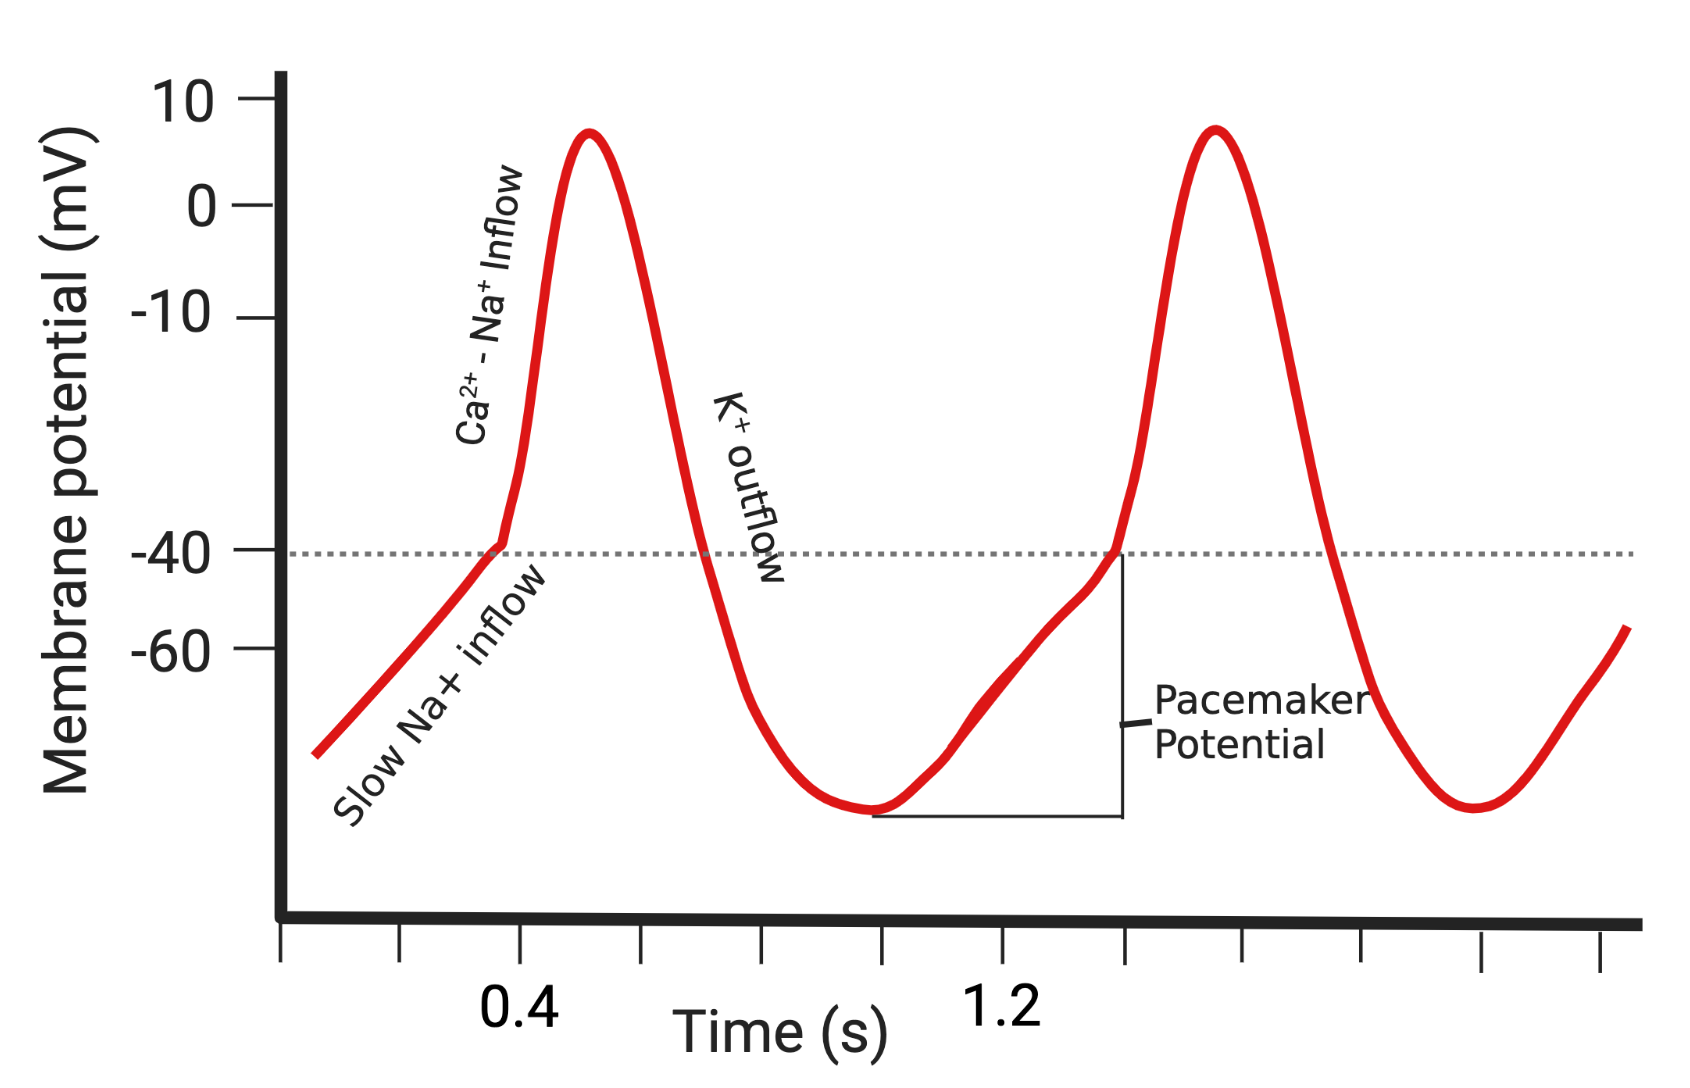
\includegraphics[width=1\linewidth]{./figure/Cardiac_SA_Node_AP.png}
    \caption{Cardiac Sino Atrial Node Excitation \footnotesize{(Created with BioRender.com)}}
    \label{fig:Cardiac_SA_Node_AP}
\end{figure}

\subsubsection{Conductivity} 

An excitation of the SA node results in full excitation of all the cardiac muscle cells, first in the atria, and then, after a delay, in the ventricles. There are three features of the myocardium that lead to this pattern of conductivity. 

\begin{figure}[!h]
    \centering
    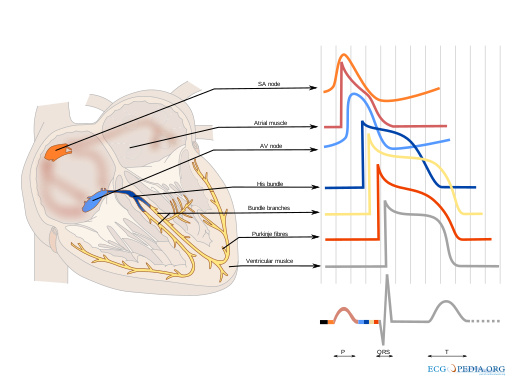
\includegraphics[width=1\linewidth]{./figure/Cardiac_Conduction.png}
    \caption{Cardiac Conduction \& Shapes of Excitation \footnotesize{(Created with BioRender.com)}}
    \label{fig:Cardiac_Conduction}
\end{figure}

First, there are specialized cardiac cells that form a conduction network. The conduction network starts with inter-nodal fibers that can rapidly carry an excitation from the SA node to the atrio-ventricular (AV) node. While carrying the excitation to the AV node the internodal fibers transmit the excitation through the atria. The excitation of the AV node and its distal conduction component, the bundle of His, is slower and delays the excitation of the ventricles. This is an important conduction component to the cardiac cycle discussed later. Once through the AV node and bundle of His the excitation travels rapidly down the right and left bundle branches out to the purkinje fibers. The branching conduction network in the ventricles is critically important to rapid and synchronous excitation of the ventricles. 

Second, there is a fibrous connective tissue boundary between the atria and the ventricles that does not transmit an excitation (does not have an excitable membrane). This helps ensure that ventricular excitation occurs only through excitation of the AV node (and no other way). THe AV node ensures that the ventricular contraction occurs after a delay so that there is time for atrial contraction to push blood into the ventricles for the final stretch of the ventricles which facilitates more tension, thus more pressure for blood flow.

Third, each excitation travels from cardiac muscle fiber to the surrounding cardiac muscle fibers due to the presence of intercalated discs that have gap junctions between cardiac muscle fibers (See Figure \ref{fig:Cardiac_Gap_Junctions}. The presence of these gap junctions not only allows, but greatly expedites the excitation of one fiber to the next. This is fundamentally different from skeletal muscle where each muscle fiber is insulated from nearby muscle fibers by the endomysium. In skeletal muscle such fiber to fiber excitation would be deleterious to controlled, coordinated movement. But in cardiac muscle this fiber to fiber wave of excitation facilitates the synchronized contraction of all atrial, and then ventricular fibers. Such "all together" contraction facilitates the change in atrial and ventricular chamber size which facilitates the change in pressure necessary for blood flow.

\begin{figure}[!h]
    \centering
    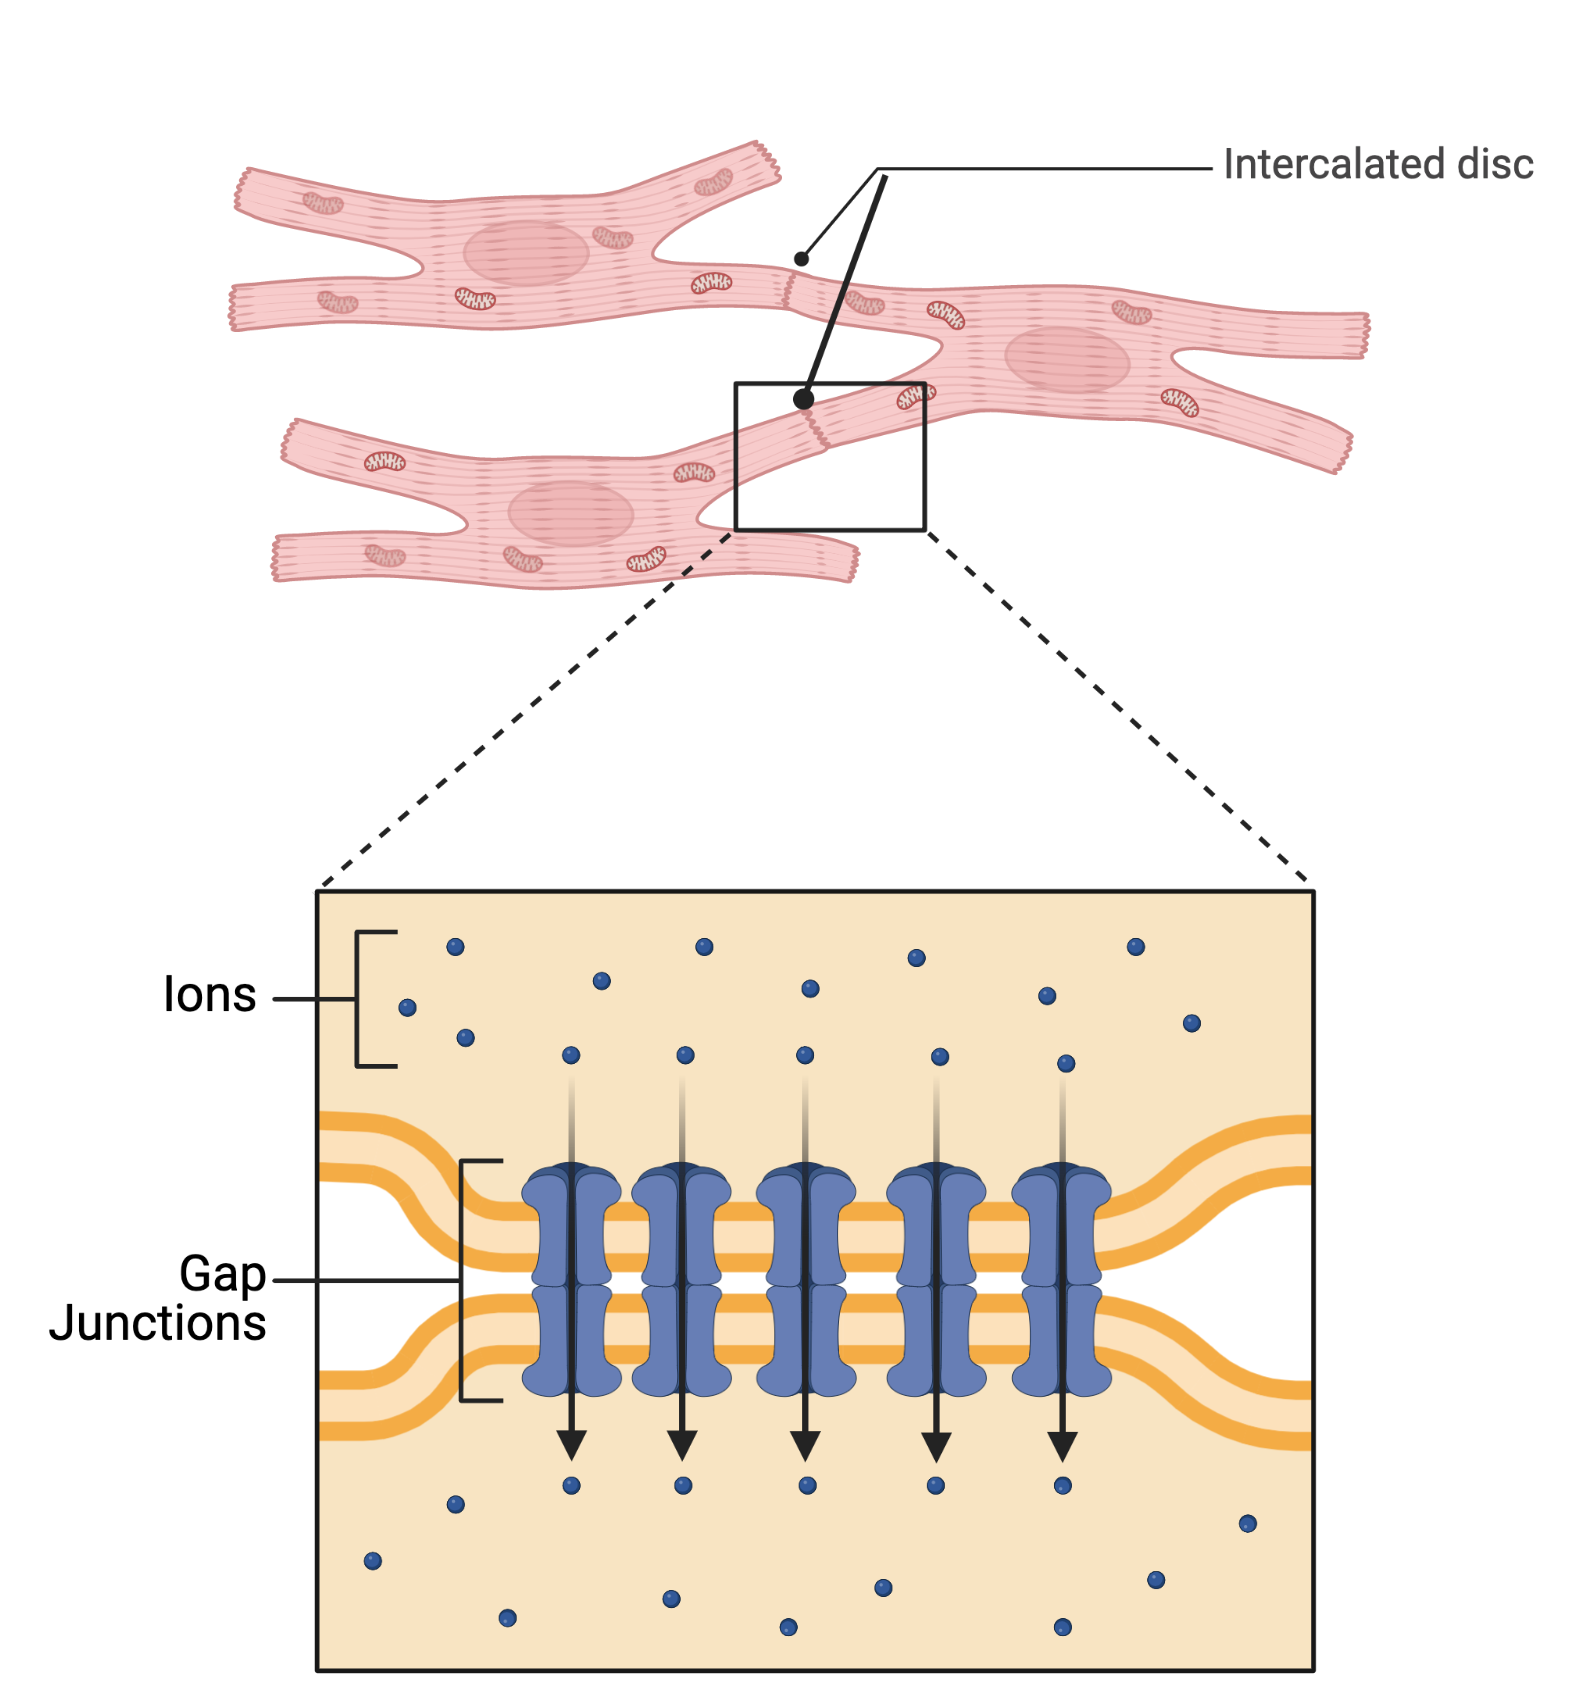
\includegraphics[width=1\linewidth]{./figure/Cardiac_Gap_Junctions.png}
    \caption{Intercalated Discs with Gap Junctions \footnotesize{(Created with BioRender.com)}}
    \label{fig:Cardiac_Gap_Junctions}
\end{figure}

% From ACH

A schematic of the cardiac conduction system and a normal electrocardiography (ECG) result are presented in Fig. 3.3. Normal conduction begins in the SA node and travels throughout the atrial myocardium (atrial depolarization) via intranodal pathways to the atrioventricular (AV) node, where it is delayed momentarily. It then travels to the bundle of His, to the bundle branches, to the Purkinje fibers, and finally to the myocardium, resulting in ventricular contraction.7 Disturbances in conduction can decrease CO (refer to the Health Conditions section for a discussion of rhythm and conduction disturbances).8

\subsubsection{Contractility}

An excitation results in a full tetany of the myocardium that generate enough tension to generate enough pressure for blood flow. For a single excitation to result in full contraction of the atria and then the ventricles requires enough $Ca^{2+}$ to be released with one excitation for tetany (not just a twitch). There are two related features that allow for this to occur in cardiac muscle. 

First, the cardiac muscle excitation (action potential) is prolonged (See Figure \ref{fig:Cardiac_Ventricular_AP}). It is prolonged due to specialized voltage gated $Ca^{2+}$ channels that allow an inward movement of $Ca^{2+}$ following the initiation of the excitation by $Na^+$. The prolonged excitation occurs all the way down to the SR which continues to release $Ca^{2+}$. Second, it has also been proposed that the prolonged SR release of $Ca^{2+}$ into the cell also contributes to the prolonged excitation of the membrane itself (a positive feedback system). 

\begin{figure}[!h]
    \centering
    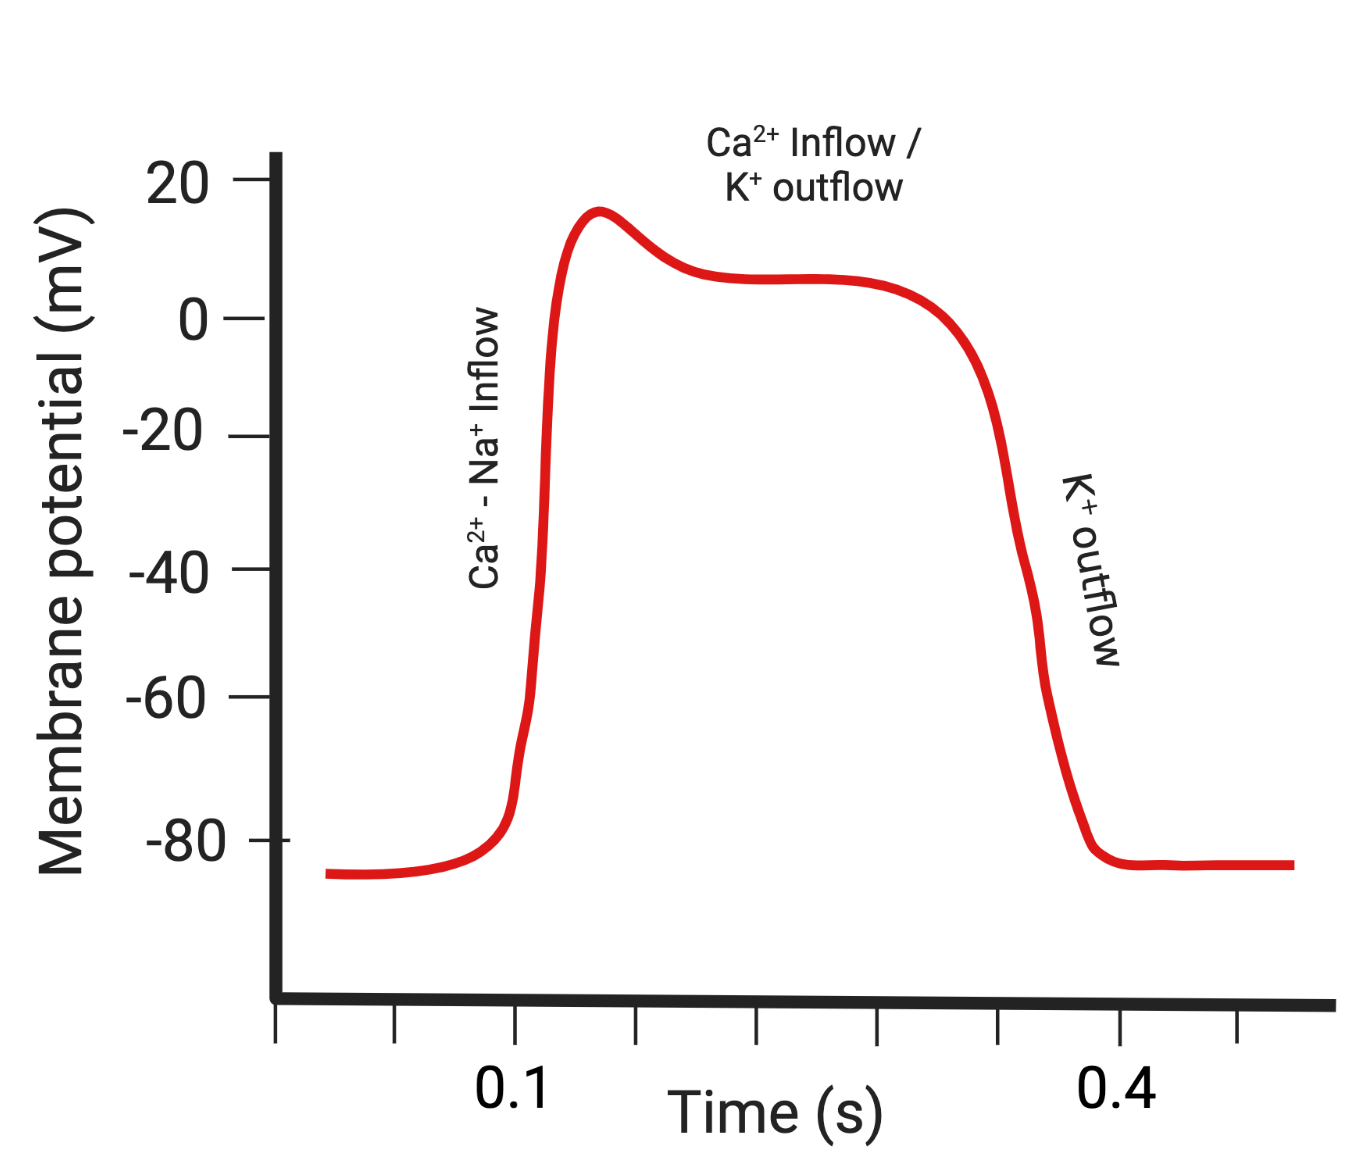
\includegraphics[width=1\linewidth]{./figure/Cardiac_Ventricular_AP.png}
    \caption{Ventricular Excitation \footnotesize{(Created with BioRender.com)}}
    \label{fig:Cardiac_Ventricular_AP}
\end{figure}

The primary take away message is that an excitation of a cardiac muscle fiber is prolonged due to inward movement of $Ca^{2+}$ across the sarcolemma, which leads to prolonged SR release of $Ca^{2+}$ for activation that also promotes prolonged excitation. Based on the importance of $Ca^{2+}$ in both prolonged excitation and activation of cardiac muscle fibers it should be of no surprise that medications that influence $Ca^{2+}$ make up two major classes of cardiac medications ($Ca^{2+}$-channel blockers; and digitalis).


\subsection{Regulation}

Frank-Starling
Frank-Starling Mechanism.
The Frank-Starling mechanism defines the normal relationship between the length and tension of the myocardium.6 The greater the stretch on the myocardium before systole (preload), the stronger is the ventricular contraction. The length–tension relationship in skeletal muscle is based on the response of individual muscle fibers; however, relationships between cardiac muscle length and tension consist of the whole heart. Therefore length is considered in terms of volume; tension is considered in terms of pressure. A greater volume of blood returning to the heart during diastole equates to greater pressures generated initially by the heart’s contractile elements. Ultimately facilitated by elastic recoil, a greater volume of blood is ejected during systole. The effectiveness of this mechanism can be reduced in pathologic situations.4

Neuroendocrine

Reflexes
Atrial reflexes
Baro-reflexes


Introduce ejection fraction (EF), left ventricular EF (LVEF) as an indication of how well tension is developing the pressure necessary to eject blood for circulation.

Neuroendocrine - regulates active tension rate and contractility (strength of the contraction)

Passive elastic - Frank - Starling mechanism and preload influences how forcefully a contraction is

Neural Input. 
The SA node has its own inherent rate. However, neural input can influence HR, heart rate variability (HRV), and contractility through the autonomic nervous system.3,9
Parasympathetic system (vagal) neural input generally decelerates cardiac function, thus decreasing HR and contractility. Parasympathetic input travels through the vagus nerves. The right vagus nerve stimulates primarily the SA node and affects rate, whereas the left vagus nerve stimulates primarily the AV node and affects AV conduction.3,9
Sympathetic system neural input is through the thoracolumbar sympathetic system and increases HR and augment ventricular contractility, thus accelerating cardiac function.3
Endocrine Input. 
In response to physical activity or stress, a release in catecholamines increases HR, contractility, and peripheral vascular resistance for a net effect of increased cardiac function (Table 3.3).3
Local Input. 
Tissue pH, concentration of carbon dioxide (CO2), concentration of oxygen (O2), and metabolic products (e.g., lactic acid) can affect vascular tone.3 During exercise, increased levels of CO2, decreased levels of O2, decreased pH, and increased levels of lactic acid at the tissue level dilate local blood vessels and therefore increase CO distribution to that area.

\subsubsection{Cardiac Reflexes} % From ACH
Cardiac reflexes influence HR and contractility and can be divided into four general categories: baroreflex (pressure), Bainbridge reflex (stretch), chemoreflex (chemical reflex), ergoreflex (ergoreceptors). 
Baroreflexes are activated through a group of mechanoreceptors located in the heart, great vessels, and intrathoracic and cervical blood vessels. These mechanoreceptors are most plentiful in the walls of the internal carotid arteries.3 Mechanoreceptors are sensory receptors that are sensitive to mechanical changes, such as pressure and stretch. Activation of the mechanoreceptors by high pressures results in an inhibition of the vasomotor center of the medulla that increases vagal stimulation. This chain of events is known as the baroreflex and results in vasodilation, decreased HR, and decreased contractility.
Mechanoreceptors located in the right atrial myocardium respond to stretch. An increased volume in the right atrium results in an increase in pressure on the atrial wall. This reflex, known as the Bainbridge reflex, stimulates the vasomotor center of the medulla, which, in turn, increases sympathetic input and increases HR and contractility.3 Respiratory sinus arrhythmia, an increased HR during inspiration and decreased HR during expiration, may be facilitated by changes in venous return and SV caused by changes in thoracic pressure induced by the respiratory cycle. At the beginning of inspiration when thoracic pressure is decreased, venous return is greater; therefore a greater stretch is exerted on the atrial wall.10
Chemoreceptors located on the carotid and aortic bodies have a primary effect on increasing rate and depth of ventilation in response to CO2 levels, but they also have a cardiac effect. Changes in CO2 during the respiratory cycle also may result in sinus arrhythmia.3
Ergoreceptors and the ergoreflex regulates hemodynamics through activation of mechanosensitive afferents to inhibit the sustained vagal effects on the heart caused by an increase heart rate during physical loading.11


\subsection{Energetics}

Cardiac muscle is exceptionally well developed for aerobic metabolism, even more so than SO skeletal muscle fibers. Even during high intensity exercise cardiac muscle is capable of taking in lactate that is circulating in the blood and facilitating its transformation back into pyruvate and acetyl-CoA for entry into the citric acid cycle (TCA). Only when there is a lack of $O_2$ available for electron transport (ETC) do the aerobic energetic pathways not keep up with glycolosis in cardiac muscle cells. 

Cardiac muscle is so well developed for aerobic metabolism that even at rest the myocardium utilizes approximately 80\% of the $O_2$ delivered the blood. Skeletal muscle, at rest, only utilizes approximately 20\% of the $O_2$ that is delivered in the blood. This makes cardiac muscle critically dependent on increases in blood flow to provide the additional $O_2$ needed in response to increased myocardial oxygen demand (RPP).

To put this in context. If HR and SBP at rest are 60 beats per minute (bpm) and 110 mmHg then RPP is 6,600. If these values reach 180 bpm and 200 mmHg for an RPP of 36,000 there is a roughly a 5.5 fold increase in myocardial oxygen demand. To meet that demand a roughly 5 fold increase in myocardial blood flow (perfusion) must be achieved. This estimate is most accurate if these values are reached at rest (rare). If these values are achieved during exercise they are an over estimate of the actual myocardial oxygen demand. During exercise there is a significant increase in the skeletal muscle pumping action on venous circulation. Therefore there is a significant increase in venous return. Increased venous return increases preload. Increased preload increases the contribution of passive tension on cardiac contraction. The increased contribution of passive tension on cardiac contraction reduces the myocardial oxygen demand. 
Therefore, a HR of 180 and SBP of 200 at rest has a higher myocardial oxygen demand than a HR of 180 and SBP of 200 during exercise despite the same RPP because of the contribution of preload and passive tension to cardiac contractility.

\section{Cardiac Function}

\subsection{Cardiac Cycle}
Blood flow throughout the cardiac cycle depends on circulatory and cardiac pressure gradients. The right side of the heart is a low-pressure system with little vascular resistance in the pulmonary arteries, whereas the left side of the heart is a high-pressure system with high vascular resistance from the systemic circulation. The cardiac cycle is the period from the beginning of one contraction, starting with sinoatrial (SA) node depolarization, to the beginning of the next contraction. Systole is the period of contraction, and diastole is the period of relaxation. Systole and diastole can also be categorized into atrial and ventricular components:
•	Atrial diastole is the period of atrial filling. The flow of blood is directed by the higher pressure in the venous circulatory system.
•	Atrial systole is the period of atrial emptying and contraction. Initial emptying of approximately 70\% of blood occurs as a result of the initial pressure gradient between the atria and the ventricles. Atrial contraction then follows, squeezing out the remaining 30\%.3 This is commonly referred to as the atrial kick.
•	Ventricular diastole is the period of ventricular filling. It initially occurs with ease; then, as the ventricle is filled, atrial contraction is necessary to squeeze the remaining blood volume into the ventricle. The amount of stretch placed on the ventricular walls during diastole, referred to as left ventricular end diastolic pressure (LVEDP), influences the force of contraction during systole. (Refer to the Factors Affecting Cardiac Output section for a description of preload.)
•	Ventricular systole is the period of ventricular contraction. The initial contraction is isovolumic (i.e., it does not eject blood), which generates the pressure necessary to serve as the catalyst for rapid ejection of ventricular blood. The left ventricular ejection fraction (EF) represents the percent of end diastolic volume ejected during systole and is normally approximately 60\%.3


\section{Circulation}

\subsection{Cardiac Output}
CO is the quantity of blood pumped by the heart in 1 minute. Regional demands for tissue perfusion (based on local metabolic needs) compete for systemic circulation, and total CO adjusts to meet these demands. Adjustment to CO occurs with changes in heart rate (HR—chronotropic) or stroke volume (SV—inotropic).4 Normal resting CO is approximately 4 to 8 liters per minute (L/min), with a resting HR of 70 beats per minute (bpm); resting SV is approximately 71mL/beat.3 The maximum value of CO represents the functional capacity of the circulatory system to meet the demands of physical activity.4
CO also can be described relative to body mass as the cardiac index (CI), the amount of blood pumped per minute per square meter of body mass. Normal CI is between 2.5 and 4.2L/min/m2. This wide normal range makes it possible for CO to decline by almost 40\% and still remain within the normal limits. Although several factors interrupt a direct correlation between CI and functional aerobic capacity,  CI below 2.5L/min/m2 represents a marked disturbance in cardiovascular performance and is always clinically relevant.5

\subsection{Cardiac Perfusion}

For a review of the major coronary arteries, refer to Fig. 3.1. Blood is pumped to the large superficial coronary arteries during ventricular systole. At this time, myocardial contraction limits the flow of blood to the myocardium; therefore myocardial tissue is perfused during diastole.

\subsection{Systemic Circulation}
For a review of the distribution of systemic circulation, refer to Fig. 3.4. Systemic circulation is affected by total peripheral resistance (TPR), which is the resistance to blood flow by the force created by the aorta and arterial system. Two factors that contribute to resistance are (1) vasomotor tone, in which vessels dilate and constrict; and (2) blood viscosity, in which greater pressure is required to propel thicker blood. TPR, also called systemic vascular resistance, and CO influence BP.3 This relationship is illustrated in the following equation:
\subsubsection{Artery \& Arteriole Flow}

\subsubsection{Vein \&  Venuole Flow}

\subsection{Pulmonary Circulation}


\section{\textit{Connections:} Electrocardiogram}

\section{\textit{Connections:} Cardiovascular Vital Signs}
\subsection{Heart Rate} 
Palpation is the second component of the physical examination and is used to evaluate and identify the following:
•	Pulses for circulation quality, HR, and rhythm (Table 3.4, Fig. 3.6)
•	Extremities for pitting edema bilaterally (Table 3.5)
When palpating HR, counting the pulse rate for 15 seconds and multiplying by 4 is sufficient with normal rates and rhythms. If rates are faster than 100bpm or slower than 60bpm, palpate the pulse for 60 seconds. If the rhythm is irregularly irregular (e.g., during atrial fibrillation) or regularly irregular (e.g., premature ventricular contractions [PVCs]), perform auscultation of heart sounds to identify the apical HR for a full minute. In these cases, palpation of pulse cannot substitute for ECG analysis to monitor the patient’s rhythm, but it may alert the therapist to the onset of these abnormalities.
Use caution in palpating pulses because manual pressure on the carotid sinus may cause baroreflex drops in heart rate (HR), blood pressure (BP), or both.

HR: HR is the primary means of determining the exercise intensity level for patients who are not taking beta-blockers or who have rate-responsive pacemakers.
•	A linear relationship exists between HR and work.
•	In general, a 20- to 30-beat increase from the resting value during activity is a safe intensity level in which a patient can exercise.
•	If a patient has undergone an exercise stress test during the hospital stay, a percentage (e.g., 60%–80%) of the maximum HR achieved during the test can be calculated to determine the exercise intensity.82
•	An example of a disproportionate HR response to low-level activity (bed or seated exercises or ambulation in room) is an HR of more than 120bpm or less than 50bpm.82
•	HRR, which provides an indication of reduced parasympathetic activity and an indicator of all-cause mortality, can be used to document improvement of tolerance to functional demands.83 HRR is the absolute difference between peak HR achieved with exercise minus the HR at 60 seconds after the completion of exercise (HRR60sec).84 An abnormal HRR at 1 minute, after a treadmill test, is reported to be a decrease of 12bpm or less with a cool-down period and less than 18bpm without a cool-down period.85
•	When prescribing activity intensity for a patient taking beta-blockers, consider that HR should not exceed 20 beats above the resting HR.
•	If prescribing an activity intensity, with use of HR, for patients with an AICD, remember that the exercise target HR should be 20 to 30 beats below the threshold rate on the defibrillator.82
•	HR cannot be used to prescribe exercise status post heart transplantation secondary to denervation of the heart during transplantation.
•	Baseline HR and recent changes in medications always should be considered before beginning an exercise session.



\subsection{Blood Pressure}
BP measurement with a sphygmomanometer (cuff) and auscultation is an indirect, noninvasive measurement of the force exerted against the arterial walls during ventricular systole (systolic blood pressure [SBP]) and during ventricular diastole (diastolic blood pressure [DBP]). BP is affected by total peripheral resistance (blood volume and elasticity of arterial walls) and CO. Table 3.6 lists normal BP ranges. Occasionally, BP measurements can be performed only on certain limbs secondary to the presence of such conditions as a percutaneously inserted central catheter, arteriovenous fistula for hemodialysis, blood clots, scarring from brachial artery cutdowns, or lymphedema (e.g., status post mastectomy). BP of the upper extremity should be measured in the following manner:
1. Check for posted signs, if any, at the bedside that indicate which arm should be used in taking BP. BP variations of 5 to 10mmHg between the right and left upper extremity are considered normal. Patients with arterial compression or obstruction may have differences of more than 10 to 15mmHg.14
2. Use a properly fitting cuff. The inflatable bladder should have a width of approximately 40% and length of approximately 80% of the upper arm circumference.15
3. Position the cuff 2.5cm above the antecubital crease.
4. Rest the relaxed arm at the level of the heart.
5. To determine how high to inflate the cuff, palpate the radial pulse, inflate until no longer palpable, and note the cuff inflation pressure. Deflate the cuff.
6. Place the bell of the stethoscope gently over the brachial artery.
7. Reinflate the cuff to 30 to 40mmHg greater than the value in step 5. Then slowly deflate the cuff. Cuff deflation should occur at approximately 2 to 3mmHg per second.15
8. Listen for the onset of tapping sounds, which represents blood flow returning to the brachial artery. This is the SBP.
9. As the pressure approaches diastolic pressure, the sounds will become muffled and in 5 to 10mmHg will be completely absent. These sounds are referred to as Korotkoff sounds (Table 3.7).14,15
<B type B>
Clinical Tip
In situations when it is difficult to auscultate or to obtain a distinct diastolic blood pressure reading (DBP), the patient’s blood pressure may be noted as systolic blood pressure (SBP)/P (i.e., rn a distinct diastolic pressure, the patienttery. This is the BP.upper arm circumference.15erted central catheter, arteriovenous fistula15
Physical Therapy Considerations
•	Recording preexertion, paraexertion, and postexertion BP is important for identification of BP responses to activity. During recovery from exercise, blood vessels dilate to allow for greater blood flow to muscles. In cardiac-compromised or very deconditioned individuals, total CO may be unable to support this increased flow to the muscles and may lead to decreased output to vital areas, such as the brain.
•	If you are unable to obtain BP on the arm, the thigh is an appropriate alternative, with auscultation at the popliteal artery.
•	Falsely high readings occur if the cuff is too small or applied loosely or if the brachial artery is lower than the heart level.
•	Evaluation of BP and HR in different postures can be used to monitor orthostatic hypotension with repeat measurements on the same arm 1 to 5 minutes after position changes. The symbols that represent patient position are shown in Fig. 3.7.
•	The same extremity should be used when serial BP recordings will be compared for an evaluation of hemodynamic response.
•	A BP record is kept on the patient’s vital sign flow sheet. This is a good place to check for BP trends throughout the day and, depending on your hospital’s policy, to document BP changes during the therapy session.
•	An auscultatory gap is the disappearance of sounds between phase 1 and phase 2 and is common in patients with high BP, venous distention, and severe aortic stenosis. Its presence can create falsely low SBPs if the cuff is not inflated enough (prevented by palpating for the disappearance of the pulse before measurement), or falsely high DBPs if the therapist stops measurement during the gap (prevented by listening for the phase 3 to phase 5 transitions).13

BP: Refer to the Cardiac Evaluation section regarding BP measurements and Table 3.6 for BP ranges. A clearly disproportionate response to exercise includes SBP decrease of 10mmHg below the resting value, a hypertensive systolic response of greater than 180mmHg, or a hypertensive diastolic response of greater than 110mmHg.82 A normotensive systolic blood response should increase 5 to 12mmHg per increase in METs.86
•	If the patient is on a pacemaker that does not have rate modulation, BP response can be used to gauge intensity. Refer to the Cardiac Pacemaker Implantation and Automatic Implantable Cardiac Defibrillator section for a discussion on pacemakers.


\printbibliography[heading=subbibintoc]